\section{Rectangular Symmetry Reduction}
\label{sec:rsr}

%\begin{figure}[]
%       \begin{center}
%                       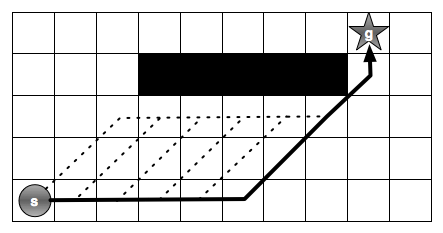
\includegraphics[scale=0.36]{diagrams/symmetry_example.png}
%       \end{center}
%       \caption{A pathfinding instance with high symmetry. We highlight the
%eventual solution returned by A* (strong line) and a number of symmetric 
%alternatives (dashed lines).}
%       \label{fig-symmetry}
%		\vspace{-0.5em}
%\end{figure}

We begin by making precise the notion of a symmetric relationship between paths
in a uniform cost graph:
\begin{definition}
\label{def:symmetry}
Two paths $\pi_{1}$ and $\pi_{2}$ are symmetric if they share the same start and
goal node and one can be derived from the other by interchanging the order of the
moves.
\end{definition}

%Consider the pathfinding instance illustrated in Figure \ref{fig-symmetry}.
%There are many symmetrical paths, some of which are marked in the figure.  With
%the popular Octile heuristic in use (which is analogous to Manhattan distance,
%but optimised for 8-connected grids) 
When applying Definition \ref{def:symmetry} to an undirected uniform cost grid 
\footnote{We say uniform but infact straight moves cost 1 and diagonal
moves cost approx. $\sqrt{2}$.} we notice that each node expanded can
often be reached from one or more of its ancestors in the search tree by several 
symmetric paths of equal length.
If the nodes on these alternative paths have an $f$-value smaller than the
current node (even an equal $f$-value is often sufficient), A* will needlessly
expand them.  
We address this problem using the high-level strategy in Algorithm
\ref{alg:rsr}; which identifies and eliminates path symmetries from the grid.

\input alg_rsr

Our approach has similarities with 4ERR~\cite{harabor10}, a symmetry breaking algorithm 
limited to 4-connected grid maps.
The main differences are: (i) we generalise 4ERR to 8-connected grid maps 
(ii) we give a stronger offline pruning operator to eliminate more nodes from
the grid (iii) we give a new online pruning operator that reduces a node's branching
factor and further speeds up search.

The generalisation to uniform-cost 8-connected grids is more challenging than it might look
at a first glance.  On a 4-connected map no node requires more than one
macro-edge (to the closest node on the opposite side of the perimeter) to retain
optimality~\cite{harabor10}.  Thus, it is easy to maintain a low branching
factor.
As we show in the next section, many more macro-edges are
needed to preserve optimality on 8-connected maps. We will identify a set of
macro-edges that is necessary and sufficient to ensure that empty rectangles can
be crossed optimally.  Keeping the branching factor within reasonable limits is
a primary motivation for the enhancements reported in the next sections.

